\documentclass[11pt]{article}
\usepackage[a4paper,top=2cm,bottom=2cm,left=3cm,right=3cm,marginparwidth=1.75cm]{geometry}
\usepackage[utf8]{inputenc}
\usepackage[german]{babel}
\usepackage{csquotes}
\usepackage[T1]{fontenc}
\usepackage{graphicx}
\usepackage{caption}
\usepackage{subcaption}
\usepackage{amsmath, amsthm, amssymb}
\usepackage{array, booktabs} 
\usepackage[table,xcdraw]{xcolor}
\usepackage[colorlinks=true, allcolors=blue]{hyperref}
\usepackage{siunitx} 
\usepackage{pgffor}
\usepackage{colortbl}
\usepackage{multicol}
\usepackage{float}
\usepackage{tabularray}

\usepackage{textcomp}
\usepackage{gensymb}
\usepackage{newunicodechar}
%\newunicodechar{°}{\degree}

\definecolor{mycolor}{RGB}{10, 173, 97}  % Green

\usepackage[backend=biber, style=authoryear, citestyle=authoryear]{biblatex}
\addbibresource{Quellen.bib}

% Bibliography disabled to avoid external biber dependency; re-enable and run biber if you need the bibliography:
% \usepackage[backend=biber, style=authoryear, citestyle=authoryear]{biblatex}
% \addbibresource{Quellen.bib}

\newcommand{\ColorTextByWavelength}[2]{%
    \WaveToPS{#1}%
    \textcolor{lambda}{#2}%
}

\begin{document}

\begin{titlepage}
   \begin{center}
       \vspace*{1cm}

       {\huge\bfseries Versuchsprotokoll}

       \vspace{1cm}

{\LARGE Franck-Hertz-Versuch}

\vspace{0.5cm}

{\Large FHZ}

\vspace{2cm}

 {Versuchsprotokoll von}
 \vspace{0.5cm}
 
{\large Alexander Ilyin, Paul Edinger}

\vspace{0.5cm}

{\small ilyia05@zedat.fu-berlin.de, paul.se@fu-berlin.de}

\vspace{1cm}


\vspace{2cm}

{\small Tutor*in: J. Sala}

\vfill

{\small Physikalisches Grundpraktikum II, WS 2024/25}

 \vspace{0.5cm}
 
 {\small Berlin, 19.02.2025}
 
 \vspace{0.5cm}
 
 {\small Freie Universität Berlin}
 
 \vspace{0.5cm}
 
 {\small Fachbereich Physik}
 
 \vspace{0.5cm}


\vspace{3cm}
            
   \end{center}
\end{titlepage}


\tableofcontents

\newpage
\section{Einführung}
Historisch war der Franck-Hertz-Versuch (1914) ein Meilenstein in der Quantenphysik, da er erstmals experimentell die Existenz diskreter Energieniveaus in Atomen bestätigte und das Bohrsche Atommodell unterstützte. Die Erkenntnisse aus diesem Experiment sind grundlegend für das Verständnis atomarer und molekularer Prozesse, die in der Materialforschung, Chemie und Quantentechnologie Anwendung finden. Der Franck-Hertz-Versuch demonstriert die Quantisierung atomarer Energieniveaus durch unelastische Elektronen-Atom-Stöße. 

In diesem Experiment wird die charakteristische Strom-Spannungs-Kurve für Quecksilberdampf (bei 150°C, 190°C, 210°C) und Neon (bei Raumtemperatur) untersucht, um Übergangsenergien, Wellenlängen und Frequenzen der emittierten Photonen zu bestimmen. Die Analyse der Kurvenverläufe bei variierten Temperaturen ermöglicht Rückschlüsse auf temperaturabhängige Effekte im Anregungsprozess.

\section{Physikalische Grundlagen} \label{grundlagen}

\begin{figure}
    \centering
    \includegraphics[width=0.5\linewidth]{Bohr_atom_model.png}
    \caption{Bohr-Modell eines Atoms: Der positiv geladene Atomkern (+Ze) ist von Elektronenschalen umgeben. Ein Elektron wechselt von der dritten auf die zweite Schale, wobei ein Photon mit der Frequenz $\nu$ emittiert wird. \cite{BohrModell}}
    \label{fig:Bohrmodell}
\end{figure}

Ein Atom besteht aus einem positiv geladenen Atomkern, der Protonen und Neutronen enthält, und einer negativ geladenen Elektronenhülle.

Nach dem \textbf{Bohrschen Atommodell} können sich Elektronen nur auf bestimmten, diskreten Bahnen oder Energieniveaus aufhalten (siehe Abbildung \ref{fig:Bohrmodell}). Diese Niveaus sind quantisiert, sodass ein Elektron nicht jede beliebige Energie annehmen kann, sondern nur bestimmte, für das jeweilige Atom charakteristische Werte. Ein Elektron auf einem höheren Energieniveau besitzt eine größere Energie als auf einem niedrigeren. Obwohl das Bohrsche Modell mittlerweile durch modernere Quantentheorien erweitert wurde, bleibt das Konzept der Energieniveaus gültig, da es sich experimentell bestätigen lässt.

Ein Elektron kann durch Energiezufuhr (z. B. durch Stöße mit anderen Elektronen) auf ein höheres Energieniveau angehoben werden. Dieser Prozess wird als \textbf{Anregung} bezeichnet. Fällt das Elektron anschließend in seinen ursprünglichen Zustand zurück, wird die zuvor aufgenommene Energie in Form eines Photons mit einer bestimmten Frequenz $f$ emittiert. Die Energie dieses Photons $E_{Ph}$ folgt der Beziehung:
\begin{align}
    E_{Ph}=hf
\end{align}
wobei $h$ das Plancksche Wirkungsquantum ist.

Stoßionisation tritt auf, wenn ein freies Elektron oder Teilchen durch einen Stoß genug kinetische Energie auf ein gebundenes Elektron überträgt, um es aus dem Atom zu lösen. Die dafür nötige Mindestenergie heißt \textbf{Ionisationsenergie} \( E_{\text{ion}} \). Mathematisch gilt:
\[
E_{\text{kin}} \geq E_{\text{ion}}.
\]
Dieser Prozess unterscheidet sich von der \textbf{Anregung}, bei der das Elektron nur ein höheres Energieniveau erreicht, ohne das Atom zu verlassen.


\subsection*{Die Franck-Hertz-Röhre}

\begin{figure}
    \centering
    \includegraphics[width=0.8\linewidth]{Schaltbild_Franck_Hertz_Versuch.png}
    \caption{Prinzipschaltbild (nicht maßstäblich) einer Franck-Hertz-Röhre (mit Glühkathode (K), Gitteranode (G), Auffängerelektrode (A), Heizspannung ($U_h$), Beschleunigungsspannung ($U_b$) und Gegenspannung ($U_g$)) \cite{SchaltbildFranckHertzVersuch}}
    \label{fig:franckhertz}
\end{figure}

Die Franck-Hertz-Röhre ist ein Experimentieraufbau, der zur experimentellen Bestätigung der Quantennatur der Energieübertragung zwischen Elektronen und Atomen dient. Sie besteht aus einer evakuierten Glasröhre, die mit einem Edelgas (z. B. Neon oder Quecksilberdampf) gefüllt ist. Im Inneren der Röhre befinden sich eine beheizte Kathode, ein Gitter und eine Auffängerelektrode (siehe Abbildung \ref{fig:franckhertz}).

Elektronen (mit der Elementarladung $e$) werden durch die thermische Emission der Kathode freigesetzt und durch eine angelegte Beschleunigungsspannung \( U_B \) in Richtung der Auffängerelektrode beschleunigt. Die kinetische Energie berechnet sich dabei:
\begin{align}
    E_{kin}=eU_B
\end{align}
Treffen die Elektronen auf Atome des Füllgases, können sie bei Erreichen einer bestimmten kinetischen Energie diese durch unelastische Stöße auf die Atome übertragen. Dies führt zur Anregung der Atome, die daraufhin Licht emittieren.

\begin{figure}
    \centering
    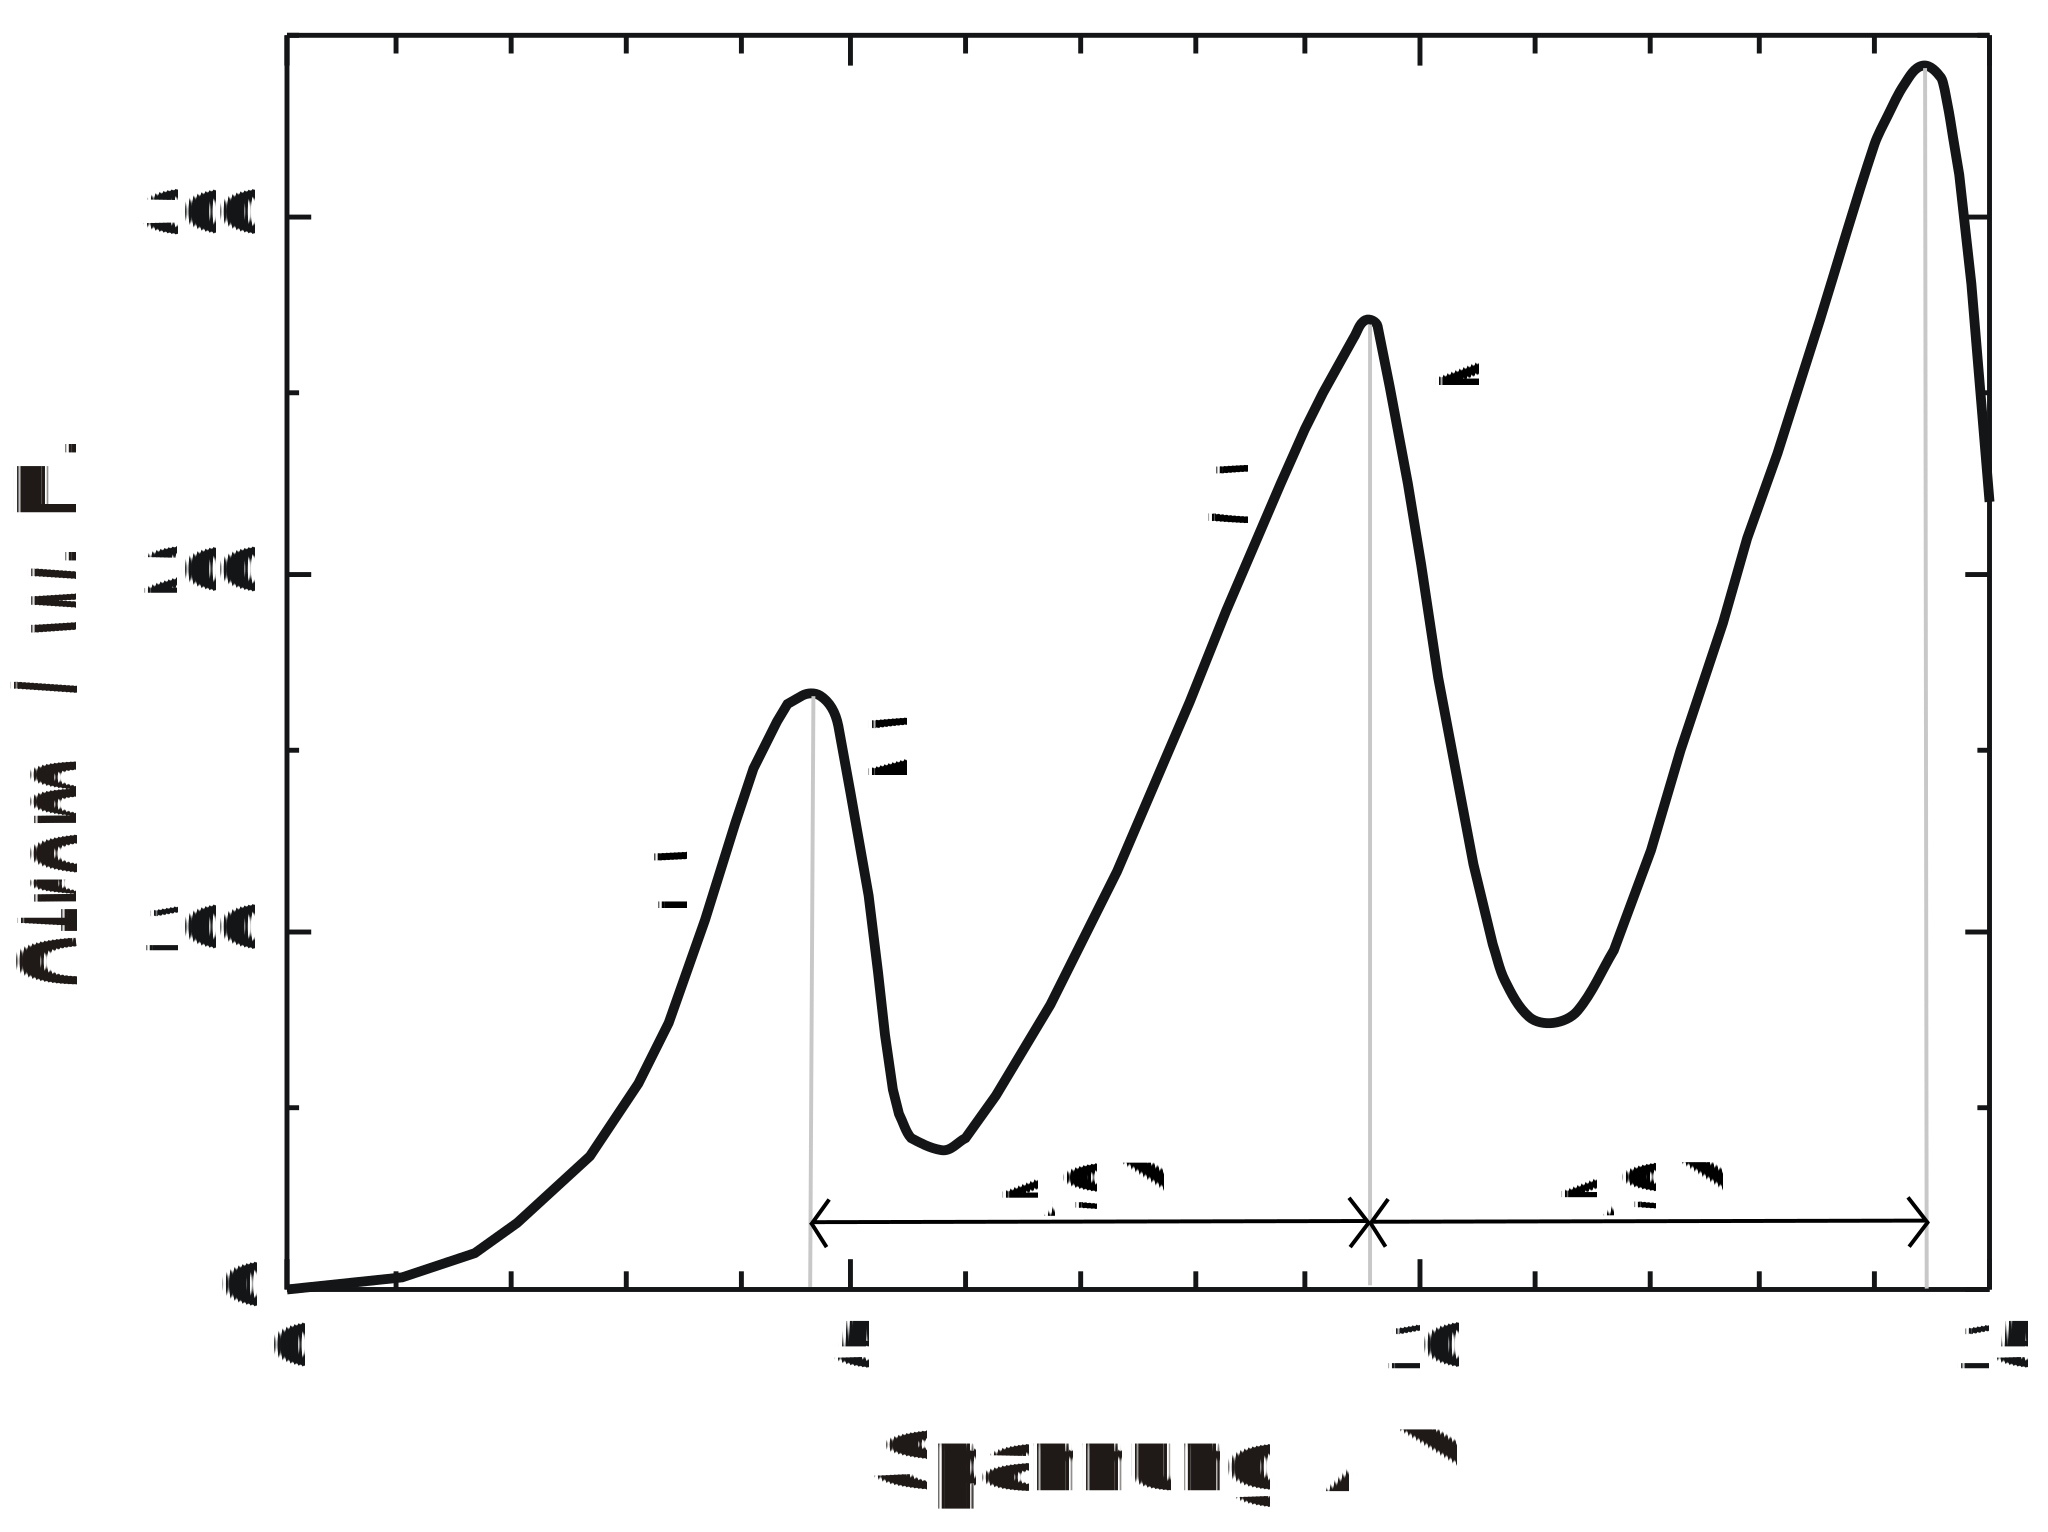
\includegraphics[width=0.6\linewidth]{Franck-Hertz_de.pdf}
    \caption{Beispielhafte Franck-Hertz-Kurve mit charakteristischen Peaks für Quecksilber (Auffängerstrom in willkürlicher Einheit (w.E.) gegenüber Beschleunigungsspannung in Volt) \cite{Franck-Hertz-Kurve-Quecksilber}}
    \label{fig:PGKurve}
\end{figure}

Die typische Form der Kurve lässt sich wie folgt beschreiben:
\begin{itemize}
    \item Bei niedrigen Beschleunigungsspannungen steigt der Strom kontinuierlich an, da die Elektronen ungehindert zur Auffängerelektrode gelangen.
    \item Ab einer kritischen Spannung \( U_1 \) tritt das erste Minimum auf, da die Elektronen ihre gesamte kinetische Energie durch unelastische Stöße verlieren.
    \item Mit weiter steigender Spannung erscheinen weitere Minima in regelmäßigen Abständen, die durch aufeinanderfolgende Anregungsprozesse entstehen.
\end{itemize}

\subsection*{Berechnung von Wellenlänge und Frequenz}
Aus den gemessenen Spannungswerten, insbesondere aus dem Abstand der Strommaxima $\Delta U$, lässt sich die Energiedifferenz $\Delta E$ der angeregten Elektronen berechnen:  

\begin{align}
    \Delta E = e \cdot \Delta U.
\end{align}

Diese Energiedifferenz entspricht der Energie der emittierten Photonen, die beim Übergang der Elektronen in einen energetisch niedrigeren Zustand freigesetzt wird:

\begin{align}
    E_{\text{Ph}} = h f = \Delta E.
\end{align}

Daraus ergibt sich für die Frequenz $f$ der emittierten Strahlung:  

\begin{align}
    f = \frac{\Delta E}{h} = \frac{e \cdot \Delta U}{h}.
\end{align}

Da die Frequenz $f$ über die Lichtgeschwindigkeit $c$ mit der Wellenlänge $\lambda$ in Zusammenhang steht, gilt:  

\begin{align}
    f = \frac{c}{\lambda}.
\end{align}

Durch Umstellen erhält man für die Wellenlänge:  

\begin{align}
    \lambda = \frac{h \cdot c}{e \cdot \Delta U}.
\end{align}

Somit kann die charakteristische Wellenlänge der emittierten Photonen aus den gemessenen Spannungswerten bestimmt werden.





\section{Aufgabenstellung}
\begin{enumerate}
    \item Elektronenstoß-Anregungskurve (Franck-Hertz-Kurve) von Quecksilber bei etwa 190°C mit dem Oszilloskop beobachten und durch geeignete Einstellung der experimentellen Parameter  optimieren
    \item Kurve quantitativ aufnehmen und zugehörige Übergangsenergie, Wellenlänge und Frequenz bestimmen 
    \item Weitere Anregungskurven für Temperaturen von 150°C und 210°C beobachten, registrieren und qualitativ diskutieren
    \item Franck-Hertz-Kurve für Neon bei Zimmertemperatur aufnehmen und auswerten
\end{enumerate}

(\cite{Aufgaben})


\section{Durchführung}

\subsection{Geräte}


\begin{itemize}
    \item Franck-Hertz-Röhre mit Hg-Füllung und Ofen (NEVA)
    \item Betriebsgerät Franck-Hertz (ELWE)
    \item Oszilloskop (HAMEG 2 verschiedene: HM203-5 für A1-3 und HM303-6 für A4)
    \item Termometer (PeakTech 5110)
    \item "PicoScope" mit Computer und "picoscope 6"-Software
    \item Kabel
    \item Franck-Hertz-Röhre Neon
\end{itemize}

Aufgrund begrenzter Versuchsaufbauten wurde zunächst mit Aufgabe 4, der Untersuchung der Neonröhre, begonnen. Dies führte dazu, dass diesem Aufbau mehr Zeit für die Durchführung gewidmet wurde – Zeit, die ursprünglich für die Experimente mit der Hg-Röhre vorgesehen war.

Die Messungen an der Hg-Röhre folgten später denselben Schritten, die bereits für die Neonröhre durchgeführt wurden. Entsprechend ist die Gliederung der folgenden Kapitel an der chronologischen Abfolge der Versuchsdurchführung ausgerichtet. Da viele Prozesse für den zweiten Versuchsaufbau identisch wiederholt wurden, wird in den Erklärungen zur Hg-Röhre häufig auf Kapitel \ref{df:A4} verwiesen, um Wiederholungen zu vermeiden.

\subsection{A4: FH-Kurve aufnehmen (Ne bei Zimmertemperatur)}\label{df:A4}

\begin{figure}[ht!]
    \centering
    \begin{subfigure}{0.8\textwidth}
        \centering
        \includegraphics[width=\textwidth]{Versuchsaufbau FHZ neon.jpeg}
        \caption{Beschriftetes Foto des Versuchsaufbaus (eigene Anfertigung)}
        \label{fig:versuchsaufbauA4}
    \end{subfigure}
    \hfill
    \begin{subfigure}{0.8\textwidth}
        \centering
        \includegraphics[width=\textwidth]{FHZ Schaltplan Neon.PNG}
        \caption{Schaltbild (\cite{FHZ-Skript})}
        \label{fig:schaltskizzeA4}
    \end{subfigure}
    \caption{Versuchsaufbau und Schaltbild von Aufgabe 4 (Franck-Hertz-Versuch mit Neon)}
\end{figure}

Die Neon-Frank-Hertz-Röhre wird gemäß der Beschriftung mit dem Betriebsgerät verbunden (siehe Abbildung \ref{fig:schaltskizzeA4}): Die Gitter-, Anoden-, Heizspannungs- und Kathodenkabel werden an den unteren Anschlüssen angeschlossen, während die Auffängerelektrode mit dem Messverstärker im oberen Bereich verbunden wird. Das Betriebsgerät wird auf dynamischen Betrieb gestellt. Zudem wird mit dem Thermometer die Raumtemperatur erfasst.

Die drei Ausgangssignale des Betriebsgeräts werden anschließend mit einem Oszilloskop (Modell HM 303-6) verbunden (siehe Abbildung \ref{fig:schaltskizzeA4}). Das Oszilloskop wird auf X-Y-Betrieb gestellt: Auf der X-Achse wird die Beschleunigungsspannung $U_B$ dargestellt, während auf der Y-Achse die verstärkte und durch den dynamischen Betrieb modulierte Signalspannung abgebildet wird ( $\propto I_A$, Strom an Auffängerelektrode). Die Einstellungen der Oszilloskopanzeige sowie die Werte für die Beschleunigungs-, Gegen- und Heizspannung werden so justiert, dass möglichst viele Peaks der Franck-Hertz-Kurve sichtbar werden. Dazu werden zunächst alle Spannungen kontrolliert hochgeregelt, während das Oszilloskop in einen größeren Maßstab gezoomt wird. Sobald die vollständige Franck-Hertz-Kurve erkennbar ist, erfolgt eine Feinjustierung der Spannungen, um die Anzahl der aufgelösten Peaks zu maximieren und den verfügbaren Bildschirmbereich optimal zu nutzen. Die Heizspannung weist dabei eine verzögerte Reaktion auf, und bereits geringe Änderungen beeinflussen das Messergebnis erheblich. Daher wird diese Spannung zuerst angepasst.

Zusätzlich werden die drei Ausgänge des Betriebsgeräts mit einem Picoscope verbunden, das über ein USB-Kabel mit einem Computer gekoppelt ist. In der Software Picoscope 6 wird die Kurve (wieder in X-Y-Betrieb) dargestellt und für einen Zeitraum gemessen, sodass sich periodische Messungen überlagern und eine Mittelung der Kurve erzeugt wird. Mithilfe der Hilfslinien der Software, die aus den x- und y-Achsen herausgezogen werden können und direkt die zugehörigen Werte anzeigen, werden die Peaks präzise eingegrenzt. Die Maxima werden dabei abgeschätzt und die Fehlerintervalle symmetrisch gewählt: Eine Hilfslinie wird an die eine Seite des obersten Plateaus gesetzt, die andere an die gegenüberliegende Seite. Falls ein Plateau aufgrund der begrenzten Stichprobengröße vom erwarteten Maximum abweicht, wird die weiter entfernte Hilfslinie entsprechend näher an den Mittelpunkt verschoben. Der obere Peak der Kurve sollte idealerweise genau über dem unteren Peak liegen (durch die Vielzahl der Messungen als breitere Struktur sichtbar).

Für die drei identifizierten Peaks werden die $U_B$-Werte systematisch erfasst. Dabei wird pro Peak der Wert des rechten Endes des Plateaus, der Wert des linken Endes sowie der Abstand zwischen beiden notiert, der von der Software direkt angezeigt wird. Alle erfassten Messdaten werden zudem für eine detailliertere Auswertung als TXT-Datei gespeichert (Dateiname: FHZ Neon Palex).

\subsection{A1: FH-Kurve beobachten und optimieren (Hg bei 190°C)}\label{df:A1}

\begin{figure}[ht!]
    \centering
    \begin{subfigure}{0.8\textwidth}
        \centering
        \includegraphics[width=\textwidth]{Versuchsaufbau FHZ Hg.jpeg}
        \caption{Beschriftetes Foto des Versuchsaufbaus (eigene Anfertigung)}
        \label{fig:versuchsaufbauA1}
    \end{subfigure}
    \hfill
    \begin{subfigure}{0.8\textwidth}
        \centering
        \includegraphics[width=\textwidth]{FHZ Schaltplan.PNG}
        \caption{Schaltbild (\cite{FHZ-Skript})}
        \label{fig:schaltskizzeA1}
    \end{subfigure}
    \caption{Versuchsaufbau und Schaltbild von Aufgabe 1 (Franck-Hertz-Versuch mit Quecksilber)}
\end{figure}

Der eingebaute Ofen der Hg-Franck-Hertz-Röhre wird auf eine Temperatur von etwa 190°C vorgeheizt. Zur präzisen Temperaturüberwachung wird ein Thermometer in die dafür vorgesehene Öffnung eingeführt.

Die Hg-Franck-Hertz-Röhre wird analog zur Neonröhre (siehe Kapitel \ref{df:A4} und Abbildung \ref{fig:schaltskizzeA1}) mit dem Betriebsgerät, dem Oszilloskop und dem Picoscope verbunden, welches über ein USB-Kabel mit einem Computer gekoppelt ist. Da sich dieser Versuchsaufbau an einem anderen Tisch befindet als jener in Aufgabe 4, kommt ein anderes Oszilloskop (Modell HM 203-5) sowie ein weiteres, jedoch baugleiches Betriebsgerät zum Einsatz.

Falls erforderlich, wird die Temperatur nachgeregelt, sodass sie auf dem Thermometer einen stabilen Wert von etwa 190°C erreicht. Anschließend werden die Spannungen sowie die Anzeigeparameter des Oszilloskops so eingestellt, dass möglichst viele Peaks der Franck-Hertz-Kurve sichtbar sind (siehe Kapitel \ref{df:A4}).

\subsection{A2: FH-Kurve aufnehmen (Hg bei 190°C)}\label{df:A2}

Aufbauend auf die vorherige Aufgabe, in der der Versuchsaufbau erstellt und die Franck-Hertz-Kurve optimiert wurde, werden nun die $U_B$-Werte der Peaks mithilfe der Picoscope-Software erfasst. Die Vorgehensweise entspricht dabei der in Aufgabe 4 beschriebenen Methode (siehe Kapitel \ref{df:A4}). In der Messung werden insgesamt 11 Peaks identifiziert und entsprechend ihrer $U_B$-Werte von der kleinsten bis zur größten nummeriert.

Um präzise Messwerte zu erhalten, wird die Datenerfassung so gestartet und gestoppt, dass die Temperatur der Hg-Franck-Hertz-Röhre währenddessen etwa 190°C beträgt. Da der Temperaturregler eine gewisse Ungenauigkeit aufweist und häufig eine leicht zu hohe oder zu niedrige Temperatur erzeugt, erfolgt die Messung während eines Aufwärm- oder Abkühlprozesses.

Alle erfassten Messdaten werden zusätzlich in einer TXT-Datei gespeichert, um eine detaillierte spätere Auswertung zu ermöglichen (Dateiname: FHZ Hg Palex 1).

\subsection{A3: FH-Kurven (Hg) für 150°C und 210°C registrieren}\label{df:A3}

Ergänzend dazu sollen für zwei weitere Temperaturen im Ofen Kurven aufgenommen werden. Für die jeweiligen Temperaturen – zunächst 210°C und anschließend 150°C – wird der Ofen gemäß der zuvor beschriebenen Methode aufgeheizt bzw. abgekühlt (siehe Kapitel \ref{df:A1}). Die Kurven werden erneut durch die Anpassung der Messparameter so eingestellt, dass eine maximale Anzahl klar erkennbarer Peaks dargestellt wird. Über die Picoscope 6-Software werden die Kurven auf dem Computer angezeigt und abschließend als Bilddateien zur späteren Vergleichsanalyse gespeichert (Dateinamen: FHZ Hg Palex 2 und FHZ Hg Palex 3).

\section{Auswertung}

\subsection{Bestimmung der Übergangsenergie bei Quecksilber mit Franck-Hertz-Kurve (A1)} \label{A:A1}

Mit einem Oszilloskop wurden die verschiedenen Spannungen des Franck-Hertz-Rohres aufgenommen, anschließend digitalisierte ein \emph{Picoscope} die Messwerte und speicherte sie als Dateien ab. In einer X-Y-Darstellung des Oszilloskops wurden die Beschleunigungsspannung $U_B$ und der Auffängerstrom, hier als $I_A = R \cdot U_A$ angegeben, aufgezeichnet. Da Oszilloskope Ströme nicht direkt messen können, wurde deren Proportionalität zur Spannung ausgenutzt. Der konkrete Wert von $R$ musste dabei nicht bestimmt werden, weil letztlich nur die Werte von $U_B$ von Interesse sind.

\begin{figure}[hbt!]
    \centering
    \includegraphics[width=0.95\linewidth]{plots/FHZ HG 1.pdf}
    \caption{Franck-Hertz-Kurve von Quecksilber bei $190^\circ\mathrm{C}$. Die Dicke der Punkte repräsentiert die logarithmische Konzentration überlappender Messwerte; bei größeren Punkten liegen mehr Werte übereinander. Die Auffangspannung wird in Abhängigkeit der Beschleunigungsspannung aufgetragen. Der Spline-Fit dient zur Bestimmung der Peakpositionen.}
    \label{fig:1}
\end{figure}

Da die Daten digitalisiert wurden, ist die Punkteverteilung durch die endliche Auflösung geprägt. Viele Messwerte überlagern sich, wenn über mehrere Zeiträume hinweg Daten aufgenommen werden. Um eine ausreichende Genauigkeit zu erzielen, erfolgte die Aufnahme über einen großen Zeitraum, der etwa 900\,000 Zeilen pro Datei umfasste. Für eine sinnvolle Darstellung, bei der sich teils 50 oder mehr Punkte überlagern, wurde die Punktgröße variiert und an die logarithmische Anzahl übereinanderliegender Messwerte angepasst. So zeigt sich, in welchen Bereichen sich die meisten Datenpunkte konzentrieren.


\begin{figure}[ht!]
    \centering
    \includegraphics[width=0.95\linewidth]{plots/FHZ HG 2.pdf}
    \caption{Franck-Hertz-Kurve von Quecksilber bei $210^\circ\mathrm{C}$ mit Spline-Anpassung.}
    \label{fig:2}
\end{figure}


\begin{figure}[ht!]
    \centering
    \includegraphics[width=0.95\linewidth]{plots/FHZ HG 3.pdf}
    \caption{Franck-Hertz-Kurve von Quecksilber bei $150^\circ\mathrm{C}$ mit Spline-Anpassung.}
    \label{fig:3}
\end{figure}

Bei $T = 190^\circ\mathrm{C}$ wurde eine Franck-Hertz-Kurve für Quecksilber aufgenommen (siehe Grafik \ref{fig:1}), um die Übergangsenergie der Elektronen zu bestimmen. Zusätzlich erfolgten Messungen bei $T = 210^\circ\mathrm{C}$ (Grafik \ref{fig:2}) und bei $T = 150^\circ\mathrm{C}$ (Grafik \ref{fig:3}). Die Kurven verlaufen bei allen Temperaturen ähnlich, zeigen aber Unterschiede im Bereich kleiner und hoher Spannungen. In Grafik \ref{fig:1} findet sich zwischen $U_B \approx 20\,\mathrm{V}$ und $55\,\mathrm{V}$ eine flach ansteigende, nahezu sinusförmige Struktur. Für $U_B < 20\,\mathrm{V}$ herrscht ein stärker chaotischer Bereich mit wechselnden Oszillationen, während die Kurve ab $U_B > 50\,\mathrm{V}$ stark ansteigt und den Darstellungsbereich verlässt. Insgesamt treten hier neun Peaks auf, von denen sich sieben gut analysieren lassen.

In den anderen Messungen sieht man ähnliche Muster: Bei $T = 210^\circ\mathrm{C}$ (Grafik~\ref{fig:2}) weitet sich der spannungsabhängige Bereich stärker aus, und es treten etwa elf Peaks auf. Bei $T = 150^\circ\mathrm{C}$ (Grafik~\ref{fig:3}) ist die Struktur unregelmäßiger, da die niedrigen Werte im mittleren Spannungsbereich liegen; dennoch können einige Peaks identifiziert werden. Verschiebungen der Kurven lassen sich unter anderem durch unterschiedliche Dampfdruckverhältnisse bei verschiedenen Temperaturen erklären.


%In den Messungen bei anderen Temperaturen verschieben sich die spannungsabhängigen Bereiche: Bei $T = 210^\circ\mathrm{C}$ wird der Bereich größer, bei $T = 150^\circ\mathrm{C}$ hingegen etwas kleiner. In Grafik \ref{fig:2} ist die typische Struktur einer Franck-Hertz-Kurve am deutlichsten erkennbar, allerdings werden die Minima stärker gedämpft, als es zunächst zu erwarten wäre. Links sind die Peaks etwas ausgedehnt und die Amplitude ist geringer, gehen aber schließlich in die charakteristische Struktur über. Am rechten Rand erkennt man erneut ein Abklingen außerhalb des Messbereichs. Insgesamt lassen sich hier ungefähr elf Peaks als sinnvoll nutzbar betrachten. In Grafik \ref{fig:3} unterscheidet sich der Kurvenverlauf bei $T = 150^\circ\mathrm{C}$ stärker von den anderen. Eine typische Franck-Hertz-Struktur ist nur noch bedingt zu erkennen, da die niedrigsten Werte in der Kurve nun in der Mitte statt am linken Rand liegen. Zwar lassen sich einige Peaks identifizieren, sie liegen jedoch alle in einem chaotischen Bereich, vergleichbar mit dem linken Bereich in Grafik \ref{fig:1}. Zudem steigen die Daten am rechten Ende nicht so schnell an wie bei den anderen Kurven. Die identifizierbaren Peaks liegen zudem leicht verschoben auf der $U_B$-Achse, was auf zusätzliche Effekte hindeuten könnte.

Zur exakten Peakbestimmung wurde ein Spline-Fit angewendet. Dazu wurden für jeden Spannungswert $U_B$ gemittelte $U_A$-Werte (gewichtete Mittelwerte, basierend auf der Anzahl der Datenpunkte) ermittelt. Die Positionen der Maxima ergaben sich aus der ersten und zweiten Ableitung des Splines. Dieses Verfahren bildet die tatsächlichen Kurvenverläufe recht zuverlässig nach.


\begin{figure}[ht!]
    \centering
    \includegraphics[width=0.95\linewidth]{plots/FHZ All max.pdf}
    \caption{Ermittelte Peakenergien $E_{\text{kin}} = U_A \cdot e$ in Abhängigkeit der Peaknummer. Alle Peakdaten aus den vorherigen Plots sind hier zusammengefasst. Eine lineare Regression wurde zur Bestimmung der Steigungen durchgeführt.}
    \label{fig:all}
\end{figure}

Mit den ermittelten Maxima (also den Energien, bei denen neue Lichtbänder entstehen) lässt sich ein linearer Zusammenhang erwarten. Theoretisch sollten diese Maxima bei ganzzahligen Vielfachen der Anregungsenergie liegen, weshalb ein Plot der Peakpositionen gegen ihre Peaknummer eine Gerade ergeben sollte.


Trägt man alle Peakpositionen gegen ihre Peaknummer auf (Abbildung \ref{fig:all}), so erhält man für den mittleren Bereich eine nahezu (fast perfekte) lineare Steigung. Aus einer linearen Anpassung ergeben sich folgende Übergangsenergien:
\[
E_{150^\circ\mathrm{C}} = (5{,}147 \pm 0{,}044)\,\mathrm{eV}, \quad
E_{190^\circ\mathrm{C}} = (4{,}989 \pm 0{,}030)\,\mathrm{eV}, \quad
E_{210^\circ\mathrm{C}} = (4{,}910 \pm 0{,}016)\,\mathrm{eV}.
\]
Vergleicht man dies mit dem Literaturwert von etwa $4{,}9\,\mathrm{eV}$, so stimmen die Werte bei 190\,°C und 210\,°C gut überein; beim niedriger temperierten Rohr (150\,°C) ist die Abweichung größer.

Aus
\[
\lambda = \frac{hc}{eU}
\quad \text{und} \quad
f = \frac{c}{\lambda},
\]
wobei $h$, $c$ und $e$ die Plancksche Konstante, Lichtgeschwindigkeit und Elementarladung bezeichnen, erhält man folgende Wellenlängen:
\[
\lambda_{150^\circ\mathrm{C}} = 240.9 \pm 2.1\,\mathrm{nm}, \quad
\lambda_{190^\circ\mathrm{C}} = 248.5 \pm 1.5\,\mathrm{nm}, \quad
\lambda_{210^\circ\mathrm{C}} = 252.51 \pm 0.81\,\mathrm{nm},
\]
und die dazugehörigen Frequenzen:
\[
f_{150^\circ\mathrm{C}} = (1.245 \pm 0.011)\times 10^{15} \,\mathrm{Hz}, \quad
f_{190^\circ\mathrm{C}} = (1.2064 \pm 0.0072)\times 10^{15} \,\mathrm{Hz}, \quad
f_{210^\circ\mathrm{C}} = (1.1872 \pm 0.0038)\times 10^{15} \,\mathrm{Hz}.
\]
Diese liegen im ultravioletten Bereich.

\subsection{Messfehler}
Die Verwendung eines Picoscopes bedingt eine digitale Auflösung, weshalb $U_B$ und $U_A$ in festen Schritten aufgezeichnet werden (z.B. $1{,}5748\,\mathrm{V}$ pro Schritt bei $U_B$ und $0{,}07874\,\mathrm{V}$ für $U_A$). Zusätzlich können Offset- und Kontaktpotenziale an den Elektroden zu systematischen Abweichungen führen, die sich insbesondere bei hohen oder niedrigen Temperaturen stärker bemerkbar machen. 
Außerdem wurden pro Datei zwar bis zu 900\,000 Datenpunkte aufgenommen, allerdings sind nur ein Teil davon im sinnvollen Bereich (andere Punkte sind teils Null oder negativ). Durch eine Gewichtung der mehrfach übereinanderliegenden Messwerte bei gleicher Spannung konnte dennoch ein Spline-Fit mit hoher Stabilität erstellt werden. Bei der linearen Regression zur Peakbestimmung ergeben sich statistische Fehler, die in die Unsicherheit der ermittelten Energiewerte und in die berechneten Wellenlängen bzw. Frequenzen eingehen. Eine weitergehende quantitative Fehleranalyse könnte diese Einflüsse (z.\,B. Kontaktpotenzial) noch genauer abschätzen.

Zur Berechnung der Wellenlänge und Frequenz kommt es natürlich auch zum Fehler, welchen man mit der Fehlerfortpflanzung folgendermaßen berechnen kann, wenn man die Konstanten als Fehlerfrei behandeln:

\[
\Delta\lambda = \frac{hc\Delta U}{eU^2}, \quad \Delta f = \frac{e\Delta U}{h}
\]


\subsection{Aufnahme der Neon-Franck-Hertz-Kurve (A2)}

\begin{figure}[ht!]
    \centering
    \includegraphics[width=0.95\linewidth]{plots/FHZ Neon.pdf}
    \caption{Franck-Hertz-Kurve von Neon-Gas bei $19^\circ\mathrm{C}$ mit drei deutlich erkennbaren Peaks. Angepasster Spline zur Unterstützung der Peakbestimmung.}
    \label{fig:Neon}
\end{figure}

Für Neon wurde das Franck-Hertz-Rohr bei Raumtemperatur (etwa $19^\circ\mathrm{C}$) betrieben. Da die Anregungsenergie von Neon deutlich über der von Quecksilber liegt, konnte innerhalb des gewählten Spannungsbereichs nur eine begrenzte Zahl ausgeprägter Maxima erzeugt werden (siehe Abbildung \ref{fig:Neon}). Analog zu Abschnitt \ref{A:A1} wurde ein Spline-Fit genutzt, um die Kurve zu glätten und die Peakpositionen besser zu identifizieren. Insgesamt konnten drei markante Peaks ausgemacht werden. Diese Struktur entspricht qualitativ der erwarteten Franck-Hertz-Charakteristik.

\begin{figure}[ht!]
    \centering
    \includegraphics[width=0.95\linewidth]{plots/FHZ Neon max.pdf}
    \caption{Peakpositionen in Abhängigkeit ihrer Peaknummer und lineare Regression der Neon-Franck-Hertz-Daten (aus Abbildung \ref{fig:Neon}).}
    \label{fig:Neon max}
\end{figure}

In Grafik \ref{fig:Neon max} sind die Peakenergien gegen ihre jeweilige Peaknummer aufgetragen, woraus sich bei nur drei Punkten eine gerade Linie anpassen lässt:
\[
E = (21{,}076 \pm 0{,}061)\,\mathrm{eV}.
\]
Der Literaturwert liegt bei etwa $18{,}7\,\mathrm{eV}$. Die Abweichung kann auf systematische Effekte (z.\,B. Kontaktpotenziale, begrenzte Genauigkeit der Spannungsversorgung, geringe Peakzahl) oder Fehler durch die digitale Datenerfassung zurückzuführen sein. Mit
\[
\lambda = \frac{hc}{eU}
\quad \text{und} \quad
f = \frac{c}{\lambda}
\]
erhält man für Neon ungefähr:
\[
\lambda_{Ne} = (58.83 \pm 0.17)\,\mathrm{nm}, \quad
f_{Ne} = (5.096 \pm 0.015)\times 10^{15}\,\mathrm{Hz},
\]
was im kurzwelligen UV-Bereich liegt. Trotz der größeren Abweichung zeigt die Messung qualitativ die erwarteten Schritte für inelastische Elektronenstöße, nur mit einem deutlich höheren Spannungsbedarf als bei Quecksilber.


\section{Zusammenfassung und Diskussion}

Bei diesem Experiment wurden mit Hilfe eines Franck-Hertz-Rohres verschiedene Gase (Quecksilber und Neon) bei unterschiedlichen Temperaturen und Einstellungen untersucht, um deren atomare Übergangsenergien zu bestimmen. Hierfür wurde in regelmäßigen Zeitabständen die Beschleunigungsspannung $U_B$ moduliert und über ein Oszilloskop aufgezeichnet. Da dieses nur Spannungen messen kann, wurde der Auffängerstrom der Elektronen über das Verhältnis 
\[
I_A = R \cdot U_A 
\]
bestimmt. Der Widerstandswert $R$ diente als Proportionalitätsfaktor, sodass bei der Auswertung der Kurven letztlich nur die angelegte Beschleunigungsspannung $U_B$ von zentraler Bedeutung war.

\subsection{Franck-Hertz-Kurve bei Quecksilber}
Zur Untersuchung von Quecksilbergas (im Franck-Hertz-Rohr) wurden drei verschiedene Temperaturen gewählt, nämlich 
\[
T = 150^\circ\mathrm{C}, \quad 190^\circ\mathrm{C} \quad \text{und} \quad 210^\circ\mathrm{C}.
\]
Durch Variation der Betriebsparameter (z.\,B. Heizstrom und maximale Beschleunigungsspannung) konnte man in jedem Fall mehrere ausgeprägte Maxima in der Franck-Hertz-Kurve erhalten. Die Form dieser Kurven unterscheidet sich jedoch teils deutlich voneinander, insbesondere im Bereich niedriger sowie hoher Spannungen. Eine Zunahme der Temperatur führte dabei meist zu etwas „regelmäßigeren“ und weiter in den hohen Spannungsbereich verschobenen Peaks.

\begin{itemize}
    \item Bei $T = 190^\circ\mathrm{C}$ wurde ein relativ stabiler Bereich gefunden, in dem etwa 9 Maxima detektiert werden konnten. Aus einer linearen Anpassung der Peakpositionen in Abhängigkeit ihrer Indexnummer ergab sich eine Übergangsenergie von 
    \[
    E = (4{,}99 \pm 0{,}03)\,\mathrm{eV}.
    \]
    
    \item Bei $T = 210^\circ\mathrm{C}$ ließen sich etwa 11 deutliche Peaks identifizieren. Die daraus resultierende Steigung führte zu 
    \[
    E = (4{,}91 \pm 0{,}02)\,\mathrm{eV},
    \]
    was dem Literaturwert von ca. $4{,}9\,\mathrm{eV}$ sehr nahe kommt.
    
    \item Bei $T = 150^\circ\mathrm{C}$ fielen die Ergebnisse hingegen unregelmäßiger aus. Die Kurve zeigte teils chaotische Bereiche mit unsauber ausgeprägten Peaks. Dennoch ließen sich einige Maxima fitten; diese führten auf eine Übergangsenergie von 
    \[
    E = (5{,}15 \pm 0{,}05)\,\mathrm{eV},
    \]
    was eine spürbare Abweichung vom Literaturwert darstellt.
\end{itemize}

Die beobachteten Unterschiede zwischen den Temperaturen können auf mehrere Faktoren zurückzuführen sein, darunter kontaktpotenzialabhängige Verschiebungen, veränderte Druckverhältnisse (aufgrund der Quecksilberdampfdichte) und potentielle Fehler in der Spannungsversorgung. Typischerweise können Kontaktpotenziale von bis zu einigen Zehntel Volt das Messergebnis beeinflussen; bei hohen Temperaturen und Spannungen macht sich dies besonders bemerkbar. Insgesamt zeigen die Ergebnisse aber eine gute Übereinstimmung mit dem Literaturwert von rund $4{,}9\,\mathrm{eV}$, besonders bei $190^\circ\mathrm{C}$ und $210^\circ\mathrm{C}$.

\subsection{Franck-Hertz-Kurve bei Neon}
Für Neon wurde das Franck-Hertz-Rohr bei etwa $19^\circ\mathrm{C}$ betrieben. Im Gegensatz zu Quecksilber benötigt Neon eine wesentlich höhere Anregungsenergie für elektronische Übergänge (literaturgemäß rund $18{,}7\,\mathrm{eV}$). Folglich erstreckt sich der Bereich der relevanten Beschleunigungsspannungen über deutlich größere Spannungswerte, und die Kurven können weniger Peaks aufweisen. 

In der praktischen Umsetzung traten lediglich drei gut ausgeprägte Maxima auf. Um diese noch klar abzubilden, musste der Messbereich angepasst werden. Die Auswertung mithilfe einer linearen Regression der Peakpositionen ergab:
\[
E = (21{,}08 \pm 0{,}07)\,\mathrm{eV},
\]
was von dem zu erwartenden Literaturwert von ca. $18{,}7\,\mathrm{eV}$ um etwa $3\,\mathrm{eV}$ abweicht. Dieser systematische Unterschied könnte durch folgende Faktoren verstärkt werden:

\begin{itemize}
    \item \textbf{Systematische Fehler:} Ungenauigkeiten in der Spannungsversorgung oder Offsetfehler im Oszilloskop.
    \item \textbf{Kontaktpotenziale:} Auch bei Neon können zusätzliche Elektroden-Potenziale für Verschiebungen sorgen, die sich als konstante Offsetspannung bemerkbar machen.
    \item \textbf{Geringe Anzahl an Peaks:} Nur drei Datenpunkte führen zu einer eingeschränkten statistischen Grundlage für die lineare Anpassung.
    \item \textbf{Bedingungen im Neon-Gas:} Druck- und Temperaturabweichungen verändern die Stoßwahrscheinlichkeiten und können einzelne Peaks beeinflussen.
\end{itemize}

Obwohl die Diskrepanz zum Literaturwert relativ groß erscheint, zeigt das Ergebnis qualitativ das erwartete Verhalten: Neon besitzt eine deutlich höhere Anregungsenergie als Quecksilber. Bereits eine kleine zusätzliche Offsetspannung im Bereich von $1\,\mathrm{V}$ bis $1{,}5\,\mathrm{V}$ könnte hier schnell eine Verschiebung von ein bis zwei Elektronenvolt bei der Auswertung erzeugen. 

% Bibliography omitted in this build; re-enable \printbibliography if using biblatex/biber.
\newpage

%\printbibliography

%\newpage
%
%\section{Messprotokoll}
%\foreach \n in {1,...,2}{
%    \begin{figure}[hb]
%        \centering
%        \includegraphics[width=0.795\linewidth]{Messprotokoll/FHZ_Paul_\n.jpeg}
%        \caption{Messprotokoll Paul Seite \n}
%    \end{figure}
%}
%
%\newpage
%\foreach \n in {1,...,2}{
%    \begin{figure}[hb]
%        \centering
%        \includegraphics[width=0.9\linewidth]{Messprotokoll/Alex_FHZ_\n.jpg}
%        \caption{Messprotokoll Alexander Seite \n}
%    \end{figure}
%}


\end{document}

